\documentclass[a4paper]{article}
\usepackage[a4paper,top=2cm,bottom=2cm,left=1cm,right=1cm,marginparwidth=1.75cm]{geometry}
% \usepackage[spanish]{babel}
% \selectlanguage{spanish}
% \usepackage[utf8]{inputenc}
% \usepackage[T1]{fontenc}
% \usepackage[spanish]{babel}

% \usepackage[T1]{fontenc}
\usepackage{graphicx} %Paquete para usar imagenes
\usepackage{listings}
\usepackage{xcolor}
\usepackage{tcolorbox}\usepackage{hyperref}

\definecolor{background}{HTML}{E7EBF4}
\definecolor{bg}{HTML}{1a1b26}
\definecolor{fg}{HTML}{a9b1d6}
\definecolor{comment}{HTML}{848cb5}
\definecolor{cyan}{HTML}{82aaff}
\definecolor{orange}{HTML}{ff9e64}
\definecolor{yellow}{HTML}{e9d78e}
\definecolor{purple}{HTML}{c792ea}
\definecolor{green}{HTML}{7fdbca}
\definecolor{numbers}{HTML}{9854f1}
\definecolor{keyword}{HTML}{9854f1}

\lstset{
    showspaces=false, % Evita mostrar espacios en blanco como ␣
    showstringspaces=false,
    inputencoding=utf8,
    extendedchars=true,
    literate=%
    {á}{{\'a}}1
    {é}{{\'e}}1
    {í}{{\'i}}1
    {ó}{{\'o}}1
    {ú}{{\'u}}1
    {ñ}{{\~n}}1
}
\lstdefinestyle{mystyle}{
    language=Python,
    basicstyle=\ttfamily,
    keywordstyle=\color{keyword},
    commentstyle=\color{comment},
    numbers=none,
    numberstyle=\tiny\color{numbers},
    frame=none,
    breaklines=true,
    % showstringspaces=false
    xleftmargin=0mm,
    xrightmargin=0mm,
}

\lstset{style=mystyle}

\newtcolorbox{mycodebox}[1][]{
    arc=17pt,  % Radio de las esquinas redondeadas
    colback=background,  % Color de fondo del cuadro
    boxrule=0.5pt,  % Grosor de la línea del cuadro
    colframe=background,
    width=0.8\textwidth,   % Anchura del cuadro
    % height=5cm,            % Altura del cuadro
    % breakable,
    #1  % Otras opciones personalizadas que puedas necesitar
}


\newtcolorbox{mycodeboxl}[1][]{
    arc=7pt,  % Radio de las esquinas redondeadas
    colback=background,  % Color de fondo del cuadro
    boxrule=0.5pt,  % Grosor de la línea del cuadro
    colframe=background,
    width=0.94\textwidth,   % Anchura del cuadro
    % height=5cm,            % Altura del cuadro
    % breakable,
    #1  % Otras opciones personalizadas que puedas necesitar
}

% Documento
\begin{document}
\newgeometry{left=3cm,right=3cm,top=2cm,bottom=2cm}
\begin{titlepage}

%--------------- Nuevo comendo de linea ----------------->
\newcommand{\linea}{\rule{\linewidth}{0.7mm}} 
\center
%--------------- Universidad, facultad y carrera ----------------->
\textbf{\Large UNIVERSIDAD NACIONAL DE SAN ANTONIO ABAD DEL CUSCO}\\[0.2cm]
\textbf{\Large FACULTAD DE INGENIERÍA ELÉCTRICA, ELECTRÓNICA,INFORMÁTICA Y MECÁNICA}\\[0.2cm]
\textbf{\Large INGENIERÍA INFORMÁTICA Y DE SISTEMAS\\[0.6cm]}

%--------------- Escudos png ----------------->

\includegraphics[width=8cm]{src/escudo-unsaac.png}
\vfill

%--------------- Tema ----------------->
\linea
\\[0.3cm]
% \vfill
\textbf{\LARGE Guía de Laboratorio 8 - Composición de Transformaciones}\\[0.2cm]
\linea \\
\vfill

%--------------- Integrantes ----------------->
\textit{\Large Alumno:}\\
%Integrantes del grupo
    \textbf{\large Ian Logan Will Quispe Ventura}\\
    \textit{211359}\\
    % \vfill

%--------------- Profesor y curso ----------------->
\vspace{0.3cm}
    \textit{\Large Docente:}\\
    \textbf{\large Hector Eduardo Ugarte Rojas}\\
\vspace{0.5cm}
    \textit{\Large Curso:}\\
    \textbf{\large Computación Gráfica}\\
    \vfill

\vspace{0.4cm}
    \textbf{\Large Cusco - Perú }\\
    \textbf{\large 2023 - II }\\
    \newpage
    \end{titlepage}

\restoregeometry
\newpage
% •·•·•·•·•·•••·•·•·•·•·•·•·•·•·•·•·•·•·•·•·•·•·•·•·•·•.,..,
% \section{Funcionamiento del algoritmo DDA}

\Large{\textbf{Traslación, Rotación, Escalado y Transformación de un triángulo}}\\[-0.4cm]
\begin{center}
\begin{mycodeboxl}
\begin{lstlisting}
from OpenGL.GL import *
from OpenGL.GLUT import *
from OpenGL.GLU import *

def Traslada():
    # Triangulo antes de trasladar
    glBegin(GL_TRIANGLES)
    glColor3f (0.5 , 0.3 , 0.9) # Color1
    glVertex2f(100.0, 100.0)
    glVertex2f(200.0, 100.0)
    glVertex2f(150.0, 150.0)
    glEnd()
    # Triangulo después de trasladar
    glTranslatef(200.0, 200.0, 0.0)
    glBegin(GL_TRIANGLES)
    glColor3f(0.8, 0.26, 1.0) # Color2
    glVertex3f(100.0, 100.0, 0.0)
    glVertex3f(200.0, 100.0, 0.0)
    glVertex3f(150.0, 150.0, 0.0)
    glEnd()

def Rota():
    #--triangulo antes de rotar
    glColor3f(0.5, 1.0, 0.7)
    glBegin(GL_TRIANGLES)
    glVertex2f(100.0, 100.0)
    glVertex2f(200.0, 100.0)
    glVertex2f(150.0, 150.0)
    glEnd()
    #--triangulo rotado
    glRotatef(45, 0, 0, 1)
    glBegin(GL_TRIANGLES)
    glVertex2f(100.0, 100.0)
    glVertex2f(200.0, 100.0)
    glVertex2f(150.0, 150.0)
    glEnd()
\end{lstlisting}
\end{mycodeboxl}
\end{center}
% -------------------------------------------------------------------
\newpage
\begin{center}
\begin{mycodeboxl}
\begin{lstlisting}
def Escala():
    #--triangulo antes de escalar
    glColor3f(0.5, 1.0, 0.7)
    glBegin(GL_TRIANGLES)
    glVertex2f(100.0, 100.0)
    glVertex2f(200.0, 100.0)
    glVertex2f(150.0, 150.0)
    glEnd()
    #--triangulo despues de escalar
    glScalef(2.0, 2.0, 2.0)
    glBegin(GL_TRIANGLES)
    glVertex2f(100.0, 100.0)
    glVertex2f(200.0, 100.0)
    glVertex2f(150.0, 150.0)
    glEnd()
def TransfComp():
    #--triangulo antes de rotar y trasladar
    glColor3f(0.5, 1.0, 0.7)
    glBegin(GL_TRIANGLES)
    glVertex2f(100.0, 100.0)
    glVertex2f(200.0, 100.0)
    glVertex2f(150.0, 150.0)
    glEnd()
    #--triangulo después de rotar y trasladar
    glRotatef(45, 0, 0, 1)
    glTranslatef(200.0, 200.0, 0.0)
    glBegin(GL_TRIANGLES)
    glVertex2f(100.0, 100.0)
    glVertex2f(200.0, 100.0)
    glVertex2f(150.0, 150.0)
    glEnd()
    glFlush()
def display():
    glClear(GL_COLOR_BUFFER_BIT)
    Traslada()
    Rota()
    Escala()
    TransfComp()
    glFlush()
\end{lstlisting}
\end{mycodeboxl}
\end{center}
Gráficos generados
\begin{center}
Traslación \hfil Rotación
\end{center}
\begin{center}

\includegraphics[width=9cm]{./src/traslacion.png}
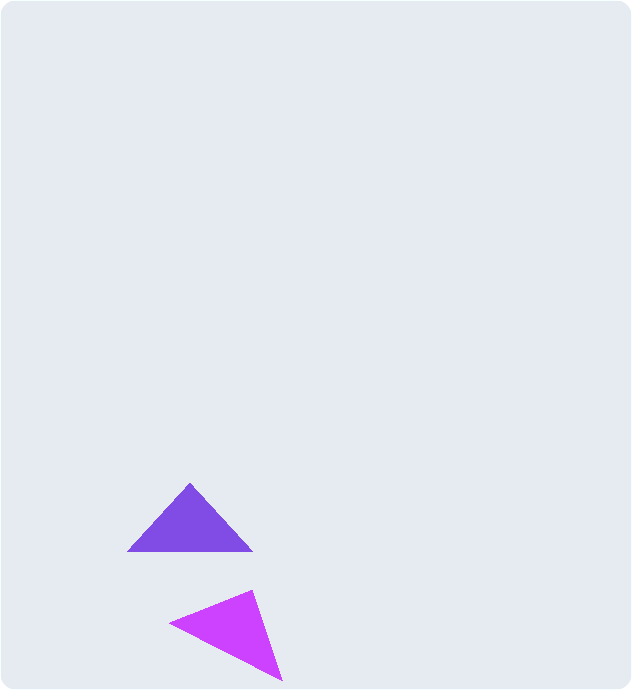
\includegraphics[width=9cm]{./src/rotacion.png}\\
\begin{center}
Escalado \hfil Transformacion 
\end{center}
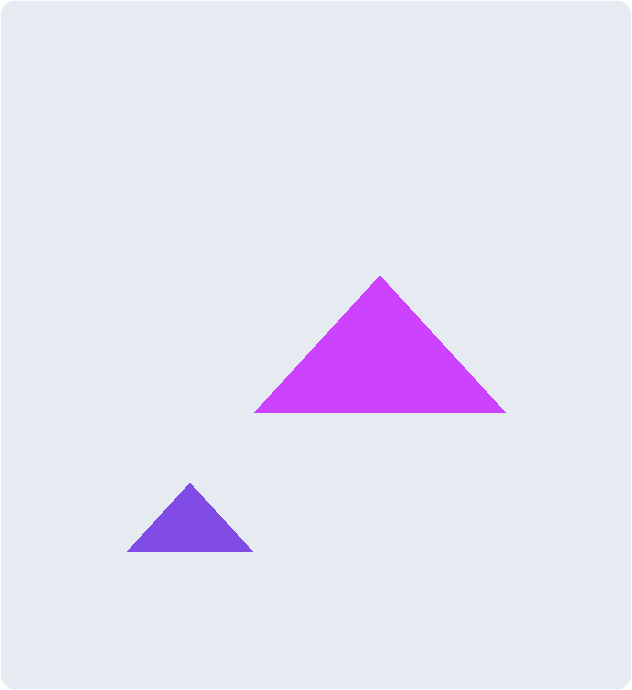
\includegraphics[width=9cm]{./src/escalado.png}
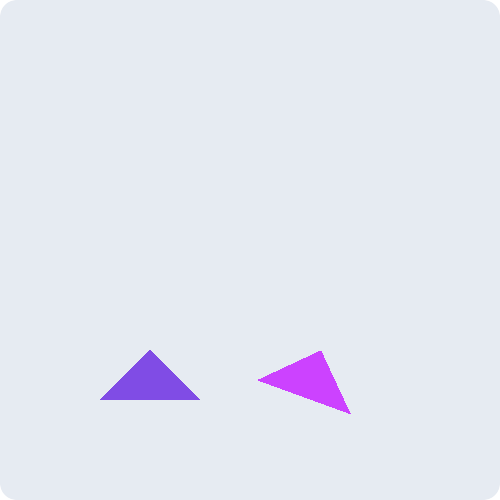
\includegraphics[width=9cm]{./src/transformacion.png}
\end{center}
% -------------------------------------------------------------------
\newpage
\Large{\textbf{Animación de la rotación y traslación de un cuadrado}}\\[-0.4cm]
\begin{center}
\begin{mycodebox}
\begin{lstlisting}
from OpenGL.GL import *
from OpenGL.GLUT import *
from OpenGL.GLU import *

angle = 0.0 
def initGL():
    glClearColor (0.9 ,0.92 , 0.95 , 1.0) # Fondo

def idle():
    global angle
    angle += 0.2
    glutPostRedisplay()

def display():
    global angle
    glClear(GL_COLOR_BUFFER_BIT)
    glMatrixMode(GL_MODELVIEW)  
    glLoadIdentity()  
    glPushMatrix() 

    # Rotar y trasladar
    glTranslatef(-0.5, 0.4, 0.0)  
    glRotatef(angle, 0.0, 0.0, 1.0)

    glBegin(GL_QUADS)
    glColor3f (0.5 , 0.3 , 0.9) # Color1
    glVertex2f(-0.3, -0.3)
    glVertex2f(0.3, -0.3)
    glVertex2f(0.3, 0.3)
    glVertex2f(-0.3, 0.3)
    glEnd()
    glPopMatrix()
    glPushMatrix() 
    # Rotar y trasladar
    glTranslatef(-0.4, -0.3, 0.0) 
    glRotatef(angle, 0.0, 0.0, 1.0) 

\end{lstlisting}
\end{mycodebox}
\end{center}
% -------------------------------------------------------------------
\newpage
\begin{center}
\begin{mycodeboxl}
\begin{lstlisting}
    glBegin(GL_QUADS)
    glColor3f(0.8, 0.26, 1.0) # Color2
    glVertex2f(-0.3, -0.3)
    glVertex2f(0.3, -0.3)
    glVertex2f(0.3, 0.3)
    glVertex2f(-0.3, 0.3)
    glEnd()
    glPopMatrix() 
    glutSwapBuffers()

def main():
    import sys
    glutInit(sys.argv)  
    glutInitDisplayMode(GLUT_DOUBLE) 
    glutInitWindowSize(540, 480)
    glutInitWindowPosition(50, 50)
    glutCreateWindow("Animation via Idle Function".encode("ascii"))
    glutDisplayFunc(display)
    glutIdleFunc(idle)  
    initGL() 
    glutMainLoop() 

if __name__ == "__main__":
    main()
\end{lstlisting}
\end{mycodeboxl}
\end{center}
\newpage
Gráfico generado 
\begin{center}

\includegraphics[width=16cm]{./src/animacion.png}
\end{center}
Animación GIF:
\url{https://gifyu.com/image/S06e4}
\newpage
% -------------------------------------------------------------------
\Large{\textbf{Escadalo (x2), Rotación (30°) y Traslacion (80, 20) de un triángulo}}\\[-0.4cm]
\begin{center}
\begin{mycodeboxl}
\begin{lstlisting}
from OpenGL.GL import *
from OpenGL.GLUT import *
from OpenGL.GLU import *

def Transformar():
    # Triangulo antes de rotar y trasladar
    glColor3f (0.5 , 0.3 , 0.9) # Color1
    glBegin(GL_TRIANGLES)
    glVertex2f(100.0, 100.0)
    glVertex2f(200.0, 100.0)
    glVertex2f(150.0, 150.0)
    glEnd()

    # Triangulo después de escalar, rotar y trasladar
    glTranslatef(80.0, 20.0, 0.0)
    glRotatef(30, 0, 0, 1)
    glScalef(2.0, 2.0, 0)

    glBegin(GL_TRIANGLES)
    glColor3f(0.8, 0.26, 1.0) # Color2
    glVertex2f(100.0, 100.0)
    glVertex2f(200.0, 100.0)
    glVertex2f(150.0, 150.0)
    glEnd()
    glFlush()

def display():
    glClear(GL_COLOR_BUFFER_BIT)
    Transformar()
    glFlush() 

def myinit():
    glClearColor (0.9 ,0.92 , 0.95 , 1.0) # Fondo
    glPointSize(1.0)
    glMatrixMode(GL_PROJECTION)
    glLoadIdentity() 
    gluOrtho2D(0.0, 499.0, 0.0, 499.0)
\end{lstlisting}
\end{mycodeboxl}
\end{center}
\begin{center}
\begin{mycodeboxl}
\begin{lstlisting}
def main():
    glutInit()
    glutInitDisplayMode(GLUT_SINGLE | GLUT_RGB)
    glutInitWindowSize(500, 500) 
    glutInitWindowPosition(0, 0)
    glutCreateWindow("Transformaciones con OpenGL")
    glutDisplayFunc(display)
    myinit()
    glutMainLoop()

if __name__ == "__main__":
    main()
\end{lstlisting}
\end{mycodeboxl}
\end{center}
Gráfico generado 
\begin{center}

\includegraphics[width=14cm]{./src/triangulo.png}
\end{center}
\newpage
% -------------------------------------------------------------------
\Large{\textbf{Traslación y Rotación de un cuadrado}}\\[-0.4cm]
\begin{center}
\begin{mycodeboxl}
\begin{lstlisting}
from OpenGL.GL import *
from OpenGL.GLUT import *
from OpenGL.GLU import *

def cuadrado():
    # Dibujar el Cuadrado 
    glBegin(GL_QUADS)
    glVertex2f(250.0, 100.0)
    glVertex2f(350.0, 100.0)
    glVertex2f(350.0, 200.0)
    glVertex2f(250.0, 200.0)
    glEnd()

def display():
    glClear(GL_COLOR_BUFFER_BIT)
    glColor3f (0.5 , 0.3 , 0.9) # Color1
    cuadrado()
    # Trasladar y rotar el cuadrado
    glRotatef(45, 0, 0, 1)
    glTranslatef(80.0, 20.0, 0.0)
    glColor3f(0.8, 0.26, 1.0) # Color2
    cuadrado()
    glFlush() 
def myinit():
    glClearColor (0.9 ,0.92 , 0.95 , 1.0) # Fondo
    glPointSize(1.0)
    glMatrixMode(GL_PROJECTION)
    glLoadIdentity() 
    gluOrtho2D(0.0, 499.0, 0.0, 499.0)
def main():
    glutInit()
    glutInitDisplayMode(GLUT_SINGLE | GLUT_RGB)
    glutInitWindowPosition(0, 0)
    glutCreateWindow("Transformaciones con OpenGL")
    glutDisplayFunc(display)
    myinit()
    glutMainLoop()
\end{lstlisting}
\end{mycodeboxl}
\end{center}
Gráfico generado 
\begin{center}
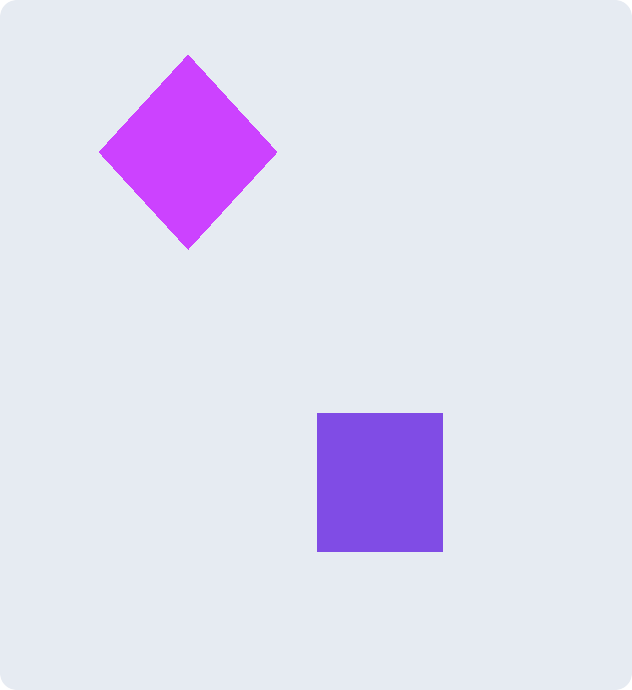
\includegraphics[width=15cm]{./src/cuadrado.png}
\end{center}
\newpage
% -------------------------------------------------------------------
\Large{\textbf{Animación de la rotación de la figura "E"}}\\[-0.4cm]
\begin{center}
\begin{mycodeboxl}
\begin{lstlisting}
from OpenGL.GL import *
from OpenGL.GLUT import *
from OpenGL.GLU import *

# Global variable
angle = 0.0  # Current rotational angle of the shapes

# Matriz de coordenadas del dibujo original
matriz_origen = [[200, 300, 300, 300, 300, 280, 200, 280],
[200, 290, 230, 290, 230, 180, 200, 180],
[200, 250, 260, 250, 260, 230, 200, 230],
[200, 200, 300, 200, 300, 180, 200, 180]]

def dibujar_E():
    glBegin(GL_QUADS)
    glColor3f(0.8, 0.26, 1.0)
    glVertex2f(matriz_origen[0][0],matriz_origen[0][1])
    glVertex2f(matriz_origen[0][2],matriz_origen[0][3])
    glVertex2f(matriz_origen[0][4],matriz_origen[0][5])
    glVertex2f(matriz_origen[0][6],matriz_origen[0][7])

    glVertex2f(matriz_origen[1][0],matriz_origen[1][1])
    glVertex2f(matriz_origen[1][2],matriz_origen[1][3])
    glVertex2f(matriz_origen[1][4],matriz_origen[1][5])
    glVertex2f(matriz_origen[1][6],matriz_origen[1][7])
\end{lstlisting}
\end{mycodeboxl}
\end{center}
\newpage

\begin{center}
\begin{mycodeboxl}
\begin{lstlisting}
    glVertex2f(matriz_origen[2][0],matriz_origen[2][1])
    glVertex2f(matriz_origen[2][2],matriz_origen[2][3])
    glVertex2f(matriz_origen[2][4],matriz_origen[2][5])
    glVertex2f(matriz_origen[2][6],matriz_origen[2][7])

    glVertex2f(matriz_origen[3][0],matriz_origen[3][1])
    glVertex2f(matriz_origen[3][2],matriz_origen[3][3])
    glVertex2f(matriz_origen[3][4],matriz_origen[3][5])
    glVertex2f(matriz_origen[3][6],matriz_origen[3][7])
    glEnd()

def initGL():
    glClearColor (0.9 ,0.92 , 0.95 , 1.0) # Fondo 
    glMatrixMode(GL_PROJECTION)
    glLoadIdentity() 
    gluOrtho2D(-499.0, 499.0, -499.0, 499.0)
def idle():
    global angle
    angle += 0.9
    glutPostRedisplay()
def display():
    global angle
    glClear(GL_COLOR_BUFFER_BIT) 
    glMatrixMode(GL_MODELVIEW)  
    glLoadIdentity() 
    glPushMatrix()
    glTranslatef(-0.25, -0.24, 0.0)
    glRotatef(angle, 0.0, 0.0, 1.0) 
    dibujar_E()
    glPopMatrix()  
    glutSwapBuffers()  
\end{lstlisting}
\end{mycodeboxl}
\end{center}
\newpage
\begin{center}
\begin{mycodeboxl}
\begin{lstlisting}
def main():
    import sys
    glutInit(sys.argv)  
    glutInitDisplayMode(GLUT_DOUBLE)
    glutInitWindowSize(500, 500)
    glutInitWindowPosition(50, 50)
    glutCreateWindow("Animation via Idle Function".encode("ascii"))
    glutDisplayFunc(display)
    glutIdleFunc(idle) 
    initGL() 
    glutMainLoop()

if __name__ == "__main__":
    main()
\end{lstlisting}
\end{mycodeboxl}
\end{center}
Gráfico generado 
\begin{center}

\includegraphics[width=13cm]{./src/animacionE.png}
\end{center}
Animación GIF:
\url{https://gifyu.com/image/S06eY}
\newpage
\end{document}
